È noto dalla letteratura scientifica che alcuni metalli aerodispersi sono più strettamente legati al traffico veicolare, rispetto ad altri metalli che invece possono avere varie origini tra cui quella terrigena. In particolare antimonio Sb e rame Cu derivano dall’usura dei freni e dei contatti elettrici, \cite{iijima2008emission,iijima2009clarification}.  Per questo motivo, per l’indagine sul \textit{lockdown}, si è scelto di valutare anche l’andamento delle concentrazioni dei metalli in aria ambiente.

In regione, l’unica stazione di fondo urbano utilizzata per il monitoraggio delle concentrazioni dei metalli rimane, ad oggi, la stazione di via Cairoli (Udine). Negli ultimi anni, infatti, le concentrazioni in aria ambiente dei metalli normati (arsenico As, cadmio Cd, nichel Ni, piombo Pb) sono sempre risultate molto al di sotto della soglia di valutazione inferiore e quindi, secondo norma, non è nemmeno necessario il loro monitoraggio; inoltre, studi chemiometrici\footnote{studi chemiometrici di modellamento di classe, SIMCA, condotti in collaborazione con l’Università La Sapienza di Roma} hanno verificato che il profilo di composizione chimica del PM10 delle principali stazioni urbane della Regione è, per quanto riguarda i metalli, lo stesso in tutte le città analizzate.

Per il presente studio sono stati quindi elaborati i dati di via Cairoli di marzo 2020 che sono stati anche confrontati coi dati dei due anni precedenti, raccolti nello stesso periodo. Fra tutti i metalli analizzati si è deciso di trattare solamente quelli ben determinabili dal punto di vista analitico (almeno metà dei dati quantificabile) e/o che denotassero delle correlazioni evidenti nella matrice di correlazione (qui non riportata). I metalli selezionati sono stati antimonio Sb e rame Cu (fra loro ben correlati e indicativi del traffico veicolare) nonché ferro Fe, manganese Mn e piombo Pb (fra loro ben correlati e a loro volta ben correlati col PM10).

Le concentrazioni medie in aria ambiente calcolate nel periodo pre-\textit{lockdown} (2-12 marzo 2020, 6 campioni) e nel periodo di \textit{lockdown} (14-26 marzo 2020, 6 campioni) sono riportate in tabella \ref{tab:metalli}. Come si può osservare nell’ultima colonna della tabella, la diminuzione percentuale più drastica si è riscontrata proprio per Sb e Cu.

In figura \ref{fig:metalli1} si osserva il trend nel mese di marzo 2020 per quanto riguarda Sb e Cu (grafico in alto sinistra) e Fe, Mn, Pb e PM10 (grafico in alto a destra). Le concentrazioni sono state “riscalate” per singolo parametro (concentrazione n-esima / concentrazione massima) così da poter apprezzare simultaneamente gli andamenti di tutti i parametri. Come si può osservare, Sb e Cu presentano un andamento decrescente dall’inizio del mese in poi che non si osserva per gli altri metalli, che invece procedono all’unisono con le concentrazioni di PM10 (nei giorni 27-28-29 marzo si è avuto il fenomeno delle sabbie desertiche molto ben evidente nel grafico di destra). I picchi maggiori in entrambi i grafici, si verificano in concomitanza delle maggiori concentrazioni di polvere ma il trend è comunque diverso nei due casi. 

Sempre in figura \ref{fig:metalli1} si osserva invece che nel 2018 (grafico in basso a sinistra) e nel 2019 (in basso a destra) antimonio e rame presentano un trend confrontabile con quello degli altri metalli.

Al fine di catturare le variazioni della composizione del PM10 pre- e post-\textit{lockdown} tenendo in considerazione contemporaneamente tutti  i metalli analizzati, è stata condotta un’Analisi delle Componenti Principali (PCA). Si ottiene il \textit{biplot} (varianza spiegata: 94\%, di cui 63\% sulla PC1 e 31\% sulla PC2) presentato nella figura \ref{fig:metalli2}.

Emerge un’ottima separazione dei campioni di tipo “\textit{dust}” (polveri desertiche, contrassegnati con le “X” marroni, e situate a destra nel piano) da quelli di tipo urbano (a sinistra); tra questi ultimi, si nota una certa tendenza dei campioni pre-\textit{lockdown} (pallini viola) a localizzarsi nella parte alta del piano, mentre i campioni relativi al periodo di \textit{lockdown} (cerchietti azzurri) si localizzano mediamente più in basso rispetto ai precedenti. Quanto alla correlazione tra le variabili chimiche originali, si nota anche un’orientazione completamente diversa degli elementi Cu e Sb, coorientati tra loro, da quella degli altri metalli.I poligoni che racchiudono i campioni delle tre tipologie (pre-\textit{lockdown}, \textit{lockdown}, e giornate di polveri desertiche) evidenziano efficacemente la diversa natura chimica delle tre situazioni ambientali e delle relative differenti sorgenti prevalenti.

\begin{table}[ht]
    \centering
    \begin{tabular}{lrrr}
    \toprule
concentrazione&	pre-\textit{lockdown}&	\textit{lockdown}&	variazione\\
\midrule
Sb ($ng/m^3$)&	0.70	&0.46	&-34\%\\
Cu ($ng/m^3$)&	5.58	&3.00	&-46\%\\
Fe ($ng/m^3$)&	185.25	&158.79	&-14\%\\
Mn($ng/m^3$)&	8.49	&8.96	&+6\%\\
Pb ($ng/m^3$)&	3.14	&3.09	&-2\%\\
PM10 ($\mu g/m^3$)&	16.50&	14.58	&-12\%\\
\bottomrule
    \end{tabular}
    \caption[Concentrazioni di metalli nel PM10, rilevate nel marzo 2020 a Udine]{Concentrazioni di metalli nel PM10, e del PM10 stesso, rilevate nel marzo 2020 a Udine in via Cairoli}
    \label{tab:metalli}
\end{table}


\begin{figure}
    \centering
    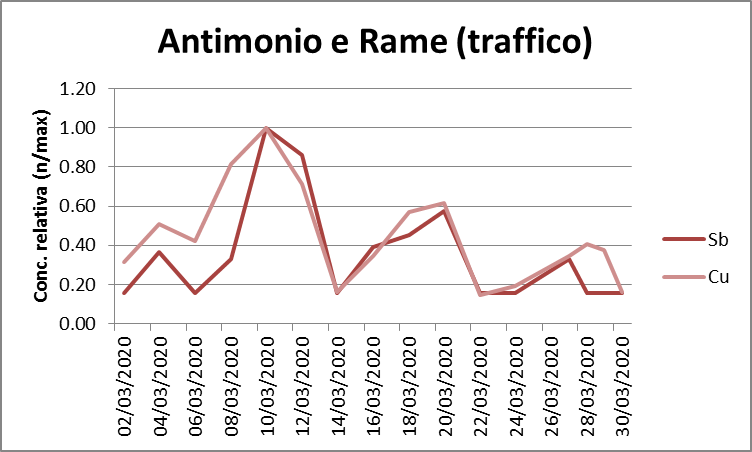
\includegraphics[width=0.45\textwidth]{figs/Sb-Cu-2020.png}
    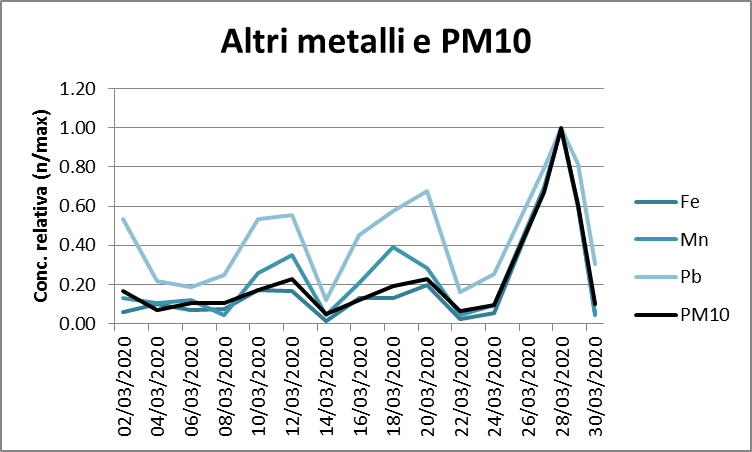
\includegraphics[width=0.45\textwidth]{figs/metalli-2020.png}\\
    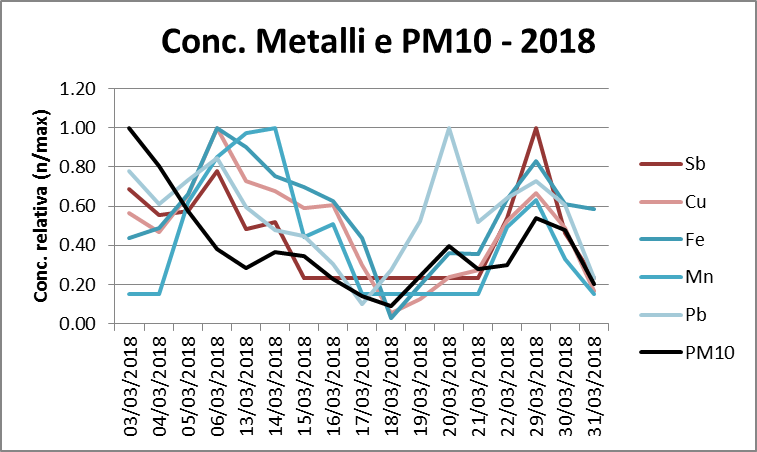
\includegraphics[width=0.45\textwidth]{figs/metalli-2018.png}
    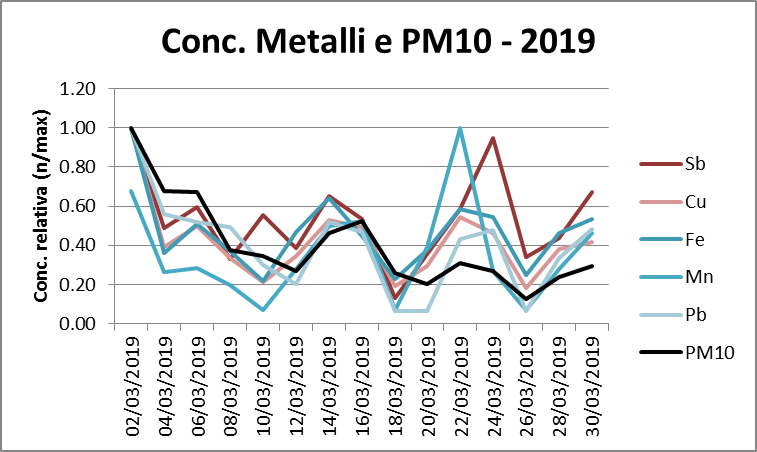
\includegraphics[width=0.45\textwidth]{figs/metalli-2019.png}
    \caption[Metalli nel PM10 a Udine]{Concentrazioni di metalli nel PM10, e del PM10 stesso, rilevate in marzo a Udine in via Cairoli e riscalate con il massimo del periodo. Sopra, a sinistra antimonio e rame, a destra ferro, manganese, piombo e PM10. Sotto, per confronto, a sinistra le concentrazioni degli stessi metalli nel marzo 2018, a destra nel marzo 2019.}
    \label{fig:metalli1}
\end{figure}

\begin{landscape}
\begin{figure}
    \centering
    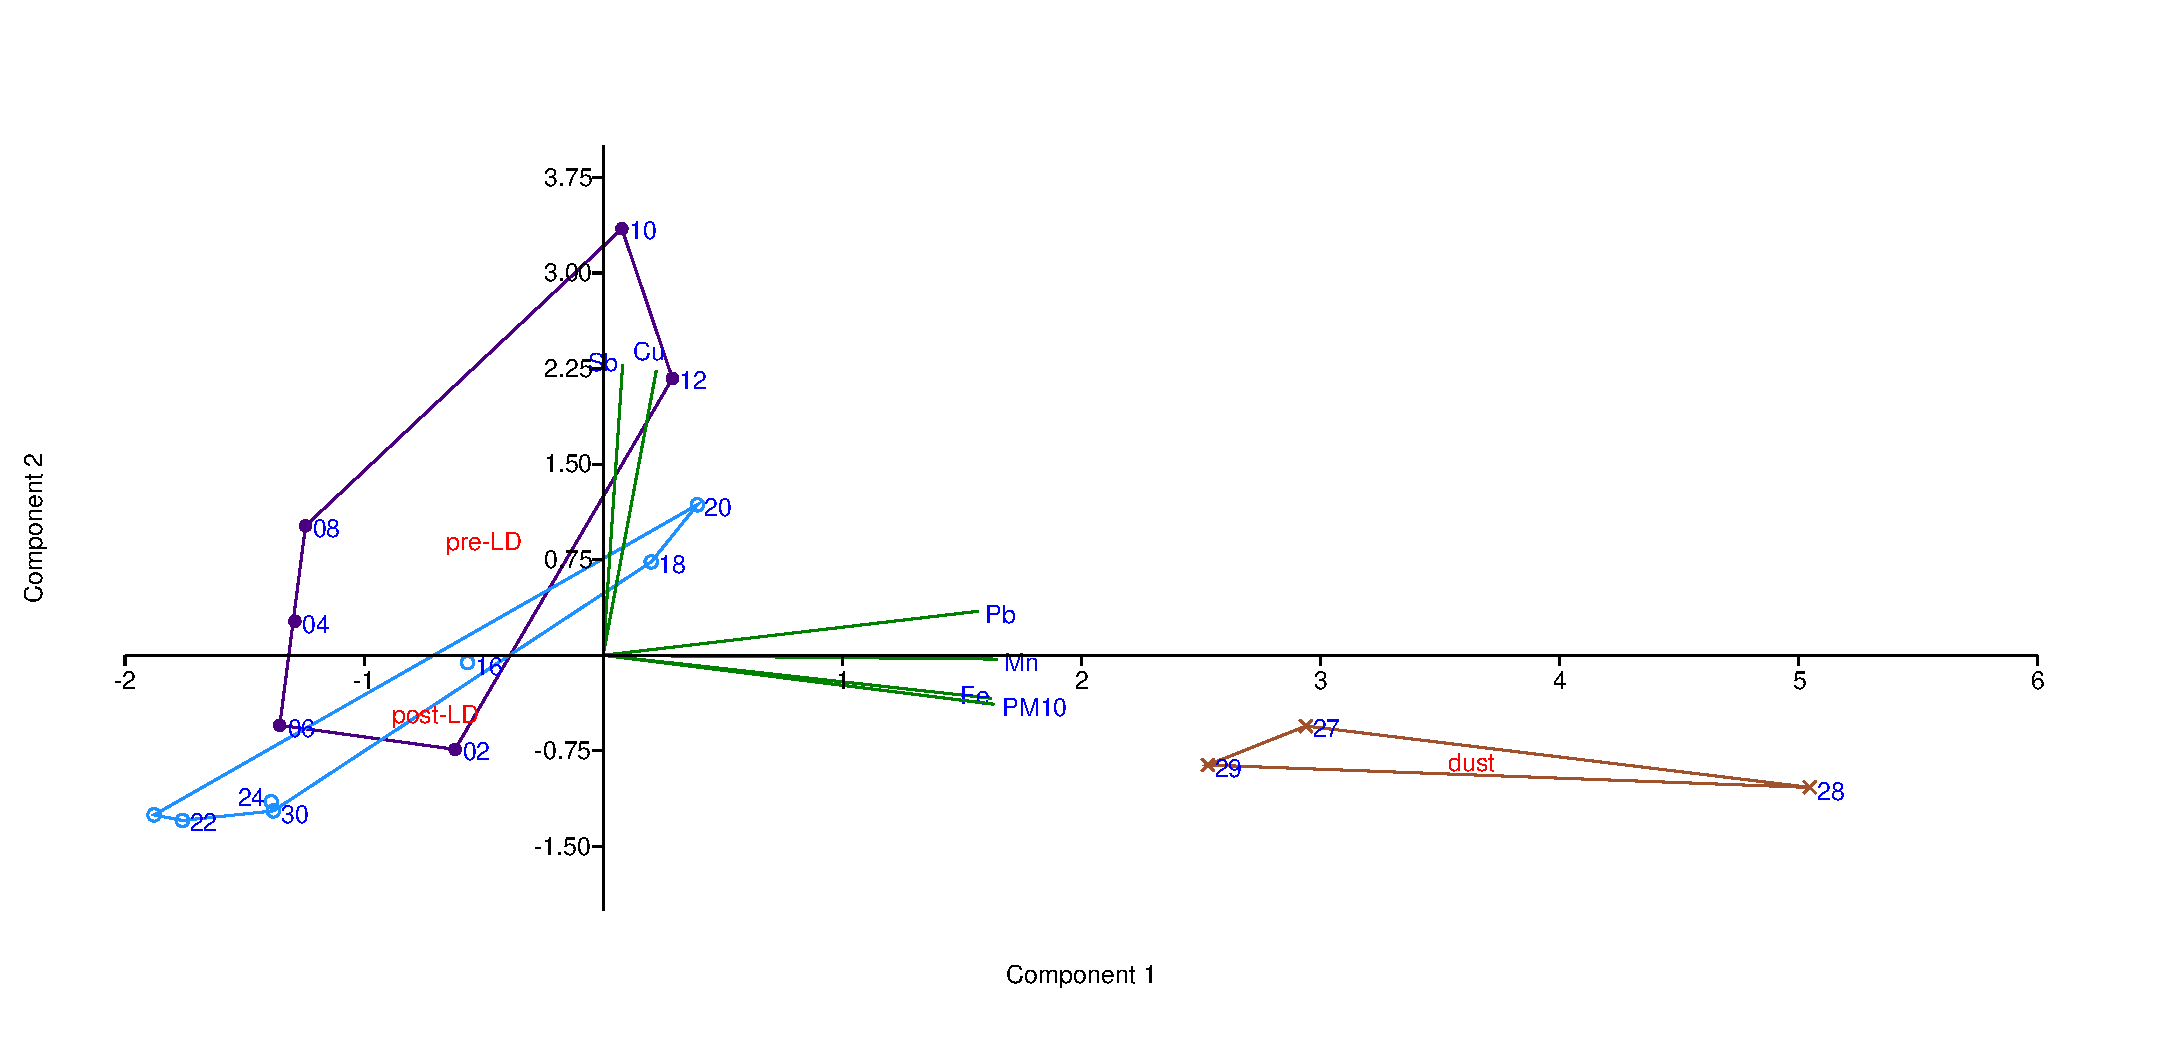
\includegraphics[width=0.9\linewidth]{figs/pca-metalli.pdf}
    \caption[PCA dei metalli nel PM10 a Udine]{Analisi delle componenti principali dei metalli nel PM10, rilevati nel marzo 2020 a Udine in via Cairoli. I numeri in blu identificano le date di campionamento. Le “X” marroni identificano i campioni raccolti nelle giornate di trasporto di polveri desertiche, i pallini viola i campioni pre-\textit{lockdown}, i cerchietti azzurri i campioni relativi al periodo di \textit{lockdown}. I vettori in verde rappresentano le proiezioni degli assi relativi alle variabili chimiche originali (\textit{loadings}).}
    \label{fig:metalli2}
\end{figure}
\end{landscape}

